\documentclass [a4paper,10pt,twocolumn]{article}
\usepackage{array,longtable}
\usepackage[dvipsnames]{color}
\usepackage[utf8]{inputenc}
\usepackage[T2A]{fontenc} 
\usepackage[english]{babel}
%\usepackage{style}
\usepackage{cmap}
\usepackage{amssymb,amsfonts,amsmath,amsthm,latexsym,amsxtra} 
\usepackage{mathtext} 
\usepackage{graphicx}
%\setlength{\textwidth}{16.5cm} \setlength{}{23.5cm}
\textwidth=18.6cm %
\textheight=26cm %

%\setlength{\topmargin}{-0.4cm} \setlength{\headheight}{0cm}

%\setlength{\headsep}{0.3cm} \evensidemargin=0.4cm
%\oddsidemargin=0.4cm
%\def\thesection{\S \arabic{section}}
\oddsidemargin=-1.3cm %
\topmargin=-1.5cm %
\setlength{\marginparsep}{0pt}
\setlength{\marginparpush}{7pt}
\setlength{\parindent}{1cm}

%\def\theequation{\arabic{section}.\arabic{equation}}
\def\R{I\kern-.20em R}
\pagestyle{empty}
%\renewcommand{\baselinestretch}{1.00} %
%\parindent 1.0em %
\thispagestyle{myheadings}

\setcounter{figure}{1}
\begin{document}
\normalsize
\protect\markright{
 \ \ \ \ \ \ \ \ \ \ \ \ \ \ \ \ \ \ \ \ \ \ \ \ \ \ \ \ \ \ \ \ \ \ \ \ \ \ \  DYRUD ET AL.: METEOR TRAIL DIFFUSION
 \setcounter{page}{2777}
}

\begin{flushleft}
\noindent\textbf{Table 1.}
Physical and simulation parameters for 105km equatorial simulation.
\end{flushleft}
\begin{tabular}{rll}
\hline
\textbf{Parameter} & & \textbf{Value}\\
\hline
External magnetic field & $B_0$ & $2.5\times 10^{-5} T$\\
Neutral gas density & $n_n$ & $5.0 \times 10^{18} m^{?3}$\\ Temperature & $T_{i,n}$ & $220 K$\\
$e^{-}$ neutral coll. freq. & $ \nu_{en}$ & $2.8\times 10^4 s^{?1}$\\
Ion mass & $m_i$ & $5.0\times 10^{?26} kg$\\
Peak/background ratio & $n_e/n_0$ & 20\\
Trail line density & $N_{line}$ & $2.0 \times 10^{14} m^{?1}$\\
Trail radius & $r_t$ & $1.0 m$\\
Ion-neutral coll. freq. & $\nu_{in}$ & $2.0 \times 10^3 s^{?1}$\\
Grid size & $n_{x,z}$ & 256\\
Grid spacing & $\Delta_{x,z}$ & $2.0 \times 10^{?2} m$\\
Time step & $\Delta_t$ & $1.0  10^{?5} s$\\
\hline
\end{tabular}

\noindent no instability exists to drive anomalous diffusion. Between 100 and 105 km, the simulation diffusion rate matches the \textbf{parallel} diffusion rate. This represents a dramatic increase in the cross-field diffusion. At 105 km, the anomalous diffusion rate exceeds the cross-field ambipolar diffusion rate by an order of magnitude. Above 105 km, the anomalous diffusion rate remains essentially flat at ~50 $m^2/s$, but well above the instability-free diffusion rate.
\subsection*{Discussion and Summary}
The simulations of meteor trails presented above show instabilities and anomalous cross-?eld diffusion. These findings have a number of implications for understanding the physics of meteor trails and interpreting meteor radar observations. The remainder of this paper discusses the physical mechanism underlying the anomalous diffusion, the minimum altitude at which instabilities appear, implications for meteor radar studies, and a summary.
\paragraph{Instability threshold} A simple calculation predicts the minimum altitude of meteor trail instabilities and anomalous diffusion. \textit{Fejer et al}. [1975] shows that the
\begin{figure}[h]
 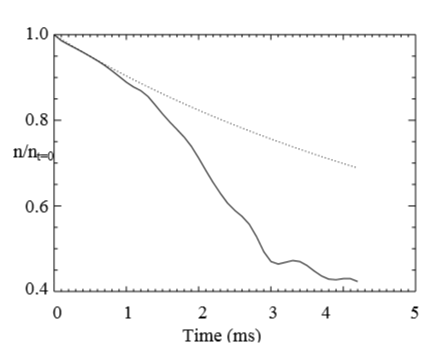
\includegraphics[width=3in]{1.PNG}
 \footnotesize\caption{Ratio of trail density to initial density vs. time from 105 km simulation. The solid line shows the average, full-width half-max, (FWHM) density from the simulation and the dashed line shows the density for a trail expanding due to cross-field ambipolar diffusion}
\end{figure}
gradient-drift instability becomes unstable when $E_\perp \cdot\triangledown n > 0$. If no large-scale electric field or neutral winds exist, then the perpendicular electric field, $E_\perp$, results solely from the cross-field ambipolar diffusion. Above 100 km, collisions dominate ion motion causing them to diffuse out of the trail. The magnetized electrons do not have sufficient mobility to follow the ions, resulting in an ambipolar electric field. Below 100 km, electron-neutral collision rates increase until the ion and electron cross-field diffusion rates are equal. At this point, $E_\perp = 0$ and no instabilities will develop to drive anomalous diffusion. Below this altitude, electrons diffuse across field lines more rapidly than ions and $E_\perp$ will have the reverse sign, damping the instability. We define a parameter, $Q$, as the ratio of electron and ion cross-field diffusion rates, $Q = T_i/T_e(\Omega_e \Omega_i/\nu_{en} \nu_{in})$, where $T_i/T_e$ usually varies between $1$ and $1/2$ and $?_e,i$ are the electron and ion cyclotron frequencies. When $Q>1, E_\perp$ points in the direction of $\triangledown n$ and the instability grows. For $Q<1$ the field reverses direction, preventing instability. Fig. 4 shows lines of $Q = 1$, the minimum altitude for instability growth, as a function of CGM latitude. For $T_i/T_e = 1$, instability is suppressed below 100 km at equatorial latitudes. For warmer electron temperatures the $Q = 1$ line indicates that instability develops at higher altitudes. This criterion for trail instability neglects the effects of external electric fields and neutral winds, both common in the E-region. It also assumes that meteor trails contain a single and moderately heavy ion species and no dust. Observed meteor trails may violate one or more of these assumptions and become unstable at lower altitudes.
\paragraph{Altitude determination} Radars frequently observe trails within a broad beam pattern, preventing an accurate determination of trail altitude. Since the decay rate of radar return power is assumed to be proportional to the trail expansion rate and since diffusion rates vary rapidly with altitude, observers use echo decay rates to infer trail altitudes [Jones,1991, @]. However, anomalous diffusion affects trail expansion rates above the $Q = 1$ altitude. In these cases, using ambipolar diffusion rates to calculate altitude may lead to errors of several kilometers.
\begin{figure}[h]
 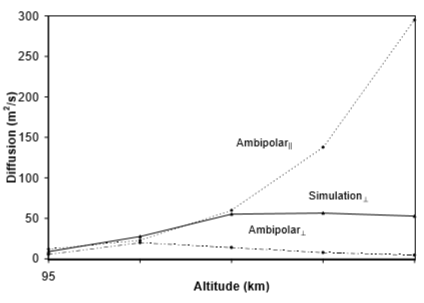
\includegraphics[width=3in]{2.PNG}
 \footnotesize\caption{Perpendicular di?usion rate from the simulation com- pared with parallel and perpendicular ambipolar di?usion rates vs. altitude.}
\end{figure}
\end{document}